\chapter{Data Sources}
\label{sec:data}

This work relies completely on all-sky surveys. All of the maps utilized are photometric-band infrared maps, except for the AME data, which is an all-sky component separation analysis product, from the Planck Collaboration's efforts to separate galactic foregrounds from the CMB.

We are primarily interested in the AKARI/IRC 9~$\mu$m band's unique coverage of the PAH bands at 6.2, 7.7, 8.6, and 11.2~$\mu$m, and if this shows any stronger/weaker correlation with AME than the WISE or IRAS 12~$\mu$m bands. In total, we use all-sky maps from 19 photometric bands, spanning the wavelength range of 6.9~$\mu$m to 550~$\mu$m***

\section{Infrared Data}

     The AKARI infrared space telescope revealed an entire sky of infrared light, from the mid to far infrared, via two instruments \citep{akari07} the Infrared Camera (IRC)\citep{irc07} and the Far Infrared Surveyor (FIS) \citep{fis07}.

     IRC's 9~$\mu$m band all-sky map demonstrates the abundance of the PAH bands carrier in the Milky Way \citep{ishihara10}. Figure \ref{fig:relSpectralResponse_MIR} shows the coverage of the MIR bands along with an example galactic cirrus SED. The 9~$\mu$m band uniquely covers major ionized PAH features at 6.2 and 7.7~$\mu$m; as well as neutral PAH features at 8.6 and 11.2~$\mu$m across the entire sky \citep{irc07}. The IRAS 12~$\mu$m band covers the 11.2 and 8.6~$\mu$m features, and the similarly-shaped WISE~12~$\mu$m band covers primarily the 11.2~$\mu$m feature. According to this distribution of PAH features across the response filters, it is expected that the IRC 9~$\mu{}$m band is most dominated by PAH emission. Figure \ref{fig:inband_ionfrac_bar} shows the relative contribution of neutral PAHs vs ionized PAHs to the AKARI/IRC 9~$\mu$m, IRAS 12~$\mu$m and WISE 12~$\mu$m bands, based on the DLO1 dust SED model. IRC 9~$\mu$m shows a larger contribution from ionized PAHs, by about 16 percent, and a conversely smaller contribution from neutral PAHs. These relative contributions remain relatively constant out to a $G_{0}$ of about 100, with the contribution from warm dust becomming a larger factor for the IRAS 12~$\mu$m and WISE 12~$\mu$m bands. Thus, according the the DL01 template, IRC 9~$\mu$m should have the highest contribution from PAHs (especially ionized) out to extreme radiation fields. Fig. \ref{fig:inband_ionfrac_ratios} demonstrates how the band ratios of the IRC 9um band vs. the other MIR bands change with different modeled PAH ionization fractions (determined using the DustEM default model template, by \cite{dustem11}.

     \begin{figure*}
     \label{fig:relSpectralResponse_MIR}
     \centering
     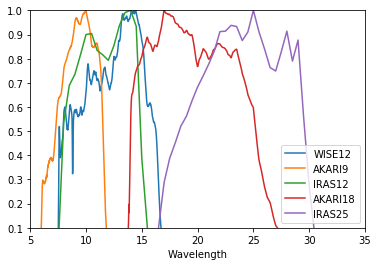
\includegraphics[width=150mm]{../Plots/RelSpectralResponse_MIR.png}
     \caption{Relative spectral response curves of the MIR bands used in this study, AKARI/IRC 9~$\mu$m, IRAS 12~$\mu$m, WISE 12~$\mu$m, AKARI 18~$\mu$m, and  IRAS 25~$\mu$m. AKARI/IRC 9~$\mu$m, IRAS 12~$\mu$m, WISE 12~$\mu$m bands are dominated by PAH emission (see Figure \ref{fig:inband_ionfrac_bar}. The AKARI 18~$\mu$m, and  IRAS 25~$\mu$m bands contain minimal PAH emission. }
     \end{figure*}


     \begin{figure*}
     \label{fig:inband_ionfrac_ratios}
     \centering
     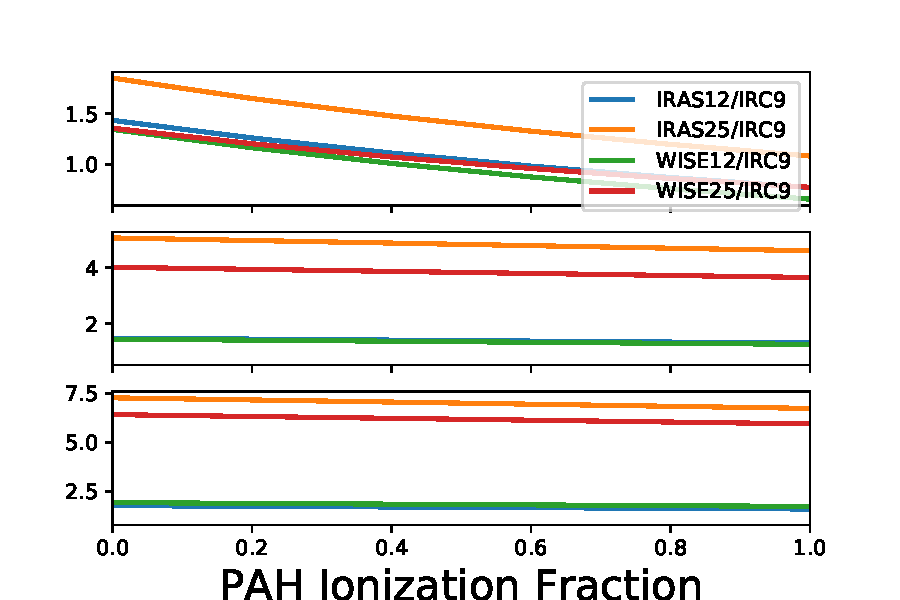
\includegraphics[width=150mm]{../Plots/band-ratio-multiple.pdf}
     \caption{Ionization fraction of PAHs vs. band ratios of IRAS12 and 25, and WISE 12 and 25~$\mu$m bads vs. the AKARI 9~$\mu$m band, for three ISRF strengths: Top: $G_{0} = 100$, Middle: $G_{0} = 1000$, and Bottom: $G_{0} = 10000$. These ratios are determined by assuming the SED template if \cite{dustem11} }
     \end{figure*}

      We utilize the most recent version of the IRC data (Ishihara, et al., in prep.) This version has had an updated model of the Zodiacal light, fitted and subtracted. The details of the improved Zodi-model, which offers an improvement over that used for the IRAS all-sky maps, are given in \cite{kondo16}.

\begin{table*}
  \label{tab:data}
  \caption{Observational data sources used in this article}
  \centering
    \begin{tabular}{lrrrrr}
    \hline\hline
    Instrument & Central Wavelength & FWHM & Uncertainty & Reference \\
    \hline
    AKARI/IRC & 9~$\mu$m  &  \~{}10$"$ & \textless 10\%   & \citep{ishihara10} \\
    AKARI/IRC & 18~$\mu$m & \~{}10$"$  & \textless 10\%     & '' \\
    AKARI/FIS & 65~$\mu$m  & 63$"$ & \textless 10\% & \citep{doi15,takita16} \\
    AKARI/FIS & 90~$\mu$m  & 78$"$ & \textless 10\%   & '' \\
    AKARI/FIS & 140~$\mu$m & 88$"$ & \textless 10\%   & '' \\
    AKARI/FIS & 160~$\mu$m & 88$"$ & \textless 10\%   & '' \\
    COBE/DIRBE & 12~$\mu$m & & & \\
    COBE/DIRBE & 25~$\mu$m & & & \\
    COBE/DIRBE & 60~$\mu$m & & & \\
    COBE/DIRBE & 100~$\mu$m & & & \\
    IRAS/IRIS & 12~$\mu$m   & 4.0$'$ &   \textless 5.1\%       & \citep{iris05} \\
    IRAS/IRIS & 25~$\mu$m   & 4.0$'$ &    \textless 15.1\%      & ''\\
    IRAS/IRIS & 60~$\mu$m   & 4.2$'$ &    \textless 10.4\%      & '' \\
    IRAS/IRIS & 100~$\mu$m  & 4.5$'$ &   \textless 13.5\%       & '' \\
    Planck/HFI & 345~$\mu$m & 4.7$'$ & & \citep{hfi14viii} \\
    Planck/HFI & 550~$\mu$m & 4.3$'$& & '' \\
    \hline
  \end{tabular}
\end{table*}

    The AKARI Far Infrared Surveyor (FIS) gives us photometric data around the peak of the typical thermal dust SED. FIS was equipped with four wavebands: two narrow bands centered at 65~$\mu$m and at 160~$\mu$m, and two wide bands at 90~$\mu$m and at 140~$\mu$m. An all-sky survey was carried out at each band \citep{kawada07}, and the processed maps have been publicly released \citep{doi15}.

     The Planck Space Observatory (Planck) High Frequency Instrument (HFI) all-sky maps, spanning 100 to 857~GHz \citep{hfi14viii} constrain the far IR dust emissivity. This study utilizes the 857~GHz (345~$\mu$m) and 545~GHz (550~$\mu$m) bands.

     Data from the Infrared Astronomical Satellite \citep{iras84} all-sky surveys are used to supplement the similarly-centered AKARI photometric bands. The IRAS 12~$\mu$m band is similar to the AKARI 9~$\mu$m band in terms of the sky coverage, central wavelength, and especially in that both surveys are heavily dominated by zodiacal light. We use the Improved Reprocessing of the IRAS Surveys (IRIS) \citep{iris05}, which use undergone a zodiacal-light removal. The Zodiacal light model, however differs between the two bands. The IRAS Zodi-subtraction is primarily based on the \cite{kelsall98} model.

\section{Planck COMMANDERAME Parameter Maps}

     We utilize the COMMANDER-Ruler astrophysical component separation maps, from the Planck Collaboration's Public Data Release 2 (hereafter, PR2). Details of the foreground contribution estimates are given in \cite{planckXII}.


     \subsection{COMMANDER-AME: Peak Frequency Distribution}

      $I_{AME}\nu_{var}$
      The Planck-COMMANDER component separation products contain estimates of known microwave foreground components (free-free, synchrotron, thermal dust emission \footnote{"Thermal dust emission" in the COMMANDER context refers to dust emission in the Rayleigh Jeans-regime, as the COMMANDER fitting does not include photometric constraints on the thermal emission peak, or consider small grain emission on the Wiens side.}) contributions to the Planck photometric bands. In addition, there is an "AME" component map, which presumes that AME originates from spinning dust. While acknowledging that such a decomposition is non-physical, the AME is further broken down into two components: a spatially varying peak frequency component, and a spatially constant peak frequency component.

      Below, we show a density plot of the peak frequencies of the varying component (I(AMEv)). The green line at 33.5 GHz indicates the peak frequency of the spatially varying component. The pink region indicates frequencies not covered by either WMAP or Planck: virtually all of the fitted peak frequncies for $AME_{var}$ are unconstrained. Only the fitted global frequency, 33.5~GHz for the spatially constant component is covered.

      The next figure shows the all-sky ratio map, of AMEvar:AMEfix. That is, the ratio of the integrated intensities of these components, rather than the intensities given directly in the COMMANDER maps. This is because the COMMANDER maps give each component's intensity at a different "reference frequency" (corresponding to photometric bands). In other words, the COMMANDER AME intensities are not peak intensities. Moreover they are intensities calculated for a single template spinning dust spectrum- but one that has been translated to fit the observations. The physical paraneters in the spinning dust model, ''spdust'' are not varied.

      For these reasons, we are very cautious in deriving conclusions from comparisons with the COMMANDE AME map. Indeed, the authors themselves include a similar disclaimer. However since there is currently no better all-sky component separation available, and carrying out a spinning dust modeling and component separation is beyond the scope of this work, we proceed with care.


\subsection{All-sky Data Processing}

      The HFI, FIS, and IRIS maps used here are downloaded from their respective online repositories, as all-sky HEALPix\footnote{HEALPix core software is described at http://healpix.sourceforge.net. The HEALPIx-based python package ``healpy'' used in this paper is associated with the following github respository: https://github.com/healpy/healpy} \citep{gorski05} NSIDE 2048 maps. In the case of the IRC maps, we first create HEALPix maps from the 4,857 all-sky survey tiles using the Aladin all-sky data visualization platform \citep{bonnarel00}. NSIDE 2048 implies an average pixel spacing of 1.7$'$. The maps are then degraded to NSIDE 1024 before carrying out a Gaussian-beam smoothing to a 1$^{\circ}$ FWHM \footnote{To be clear, maps are converted first to spherical harmonic space, smoothed, and transformed back to position space using - steps carried about by the smoothing function contained in the healpy python package \cite{healpy}}. Following the smoothing process, the maps are degraded once more to NSIDE 256, or 15arcmin pixel-width \footnote{HEALPix pixel scale rebinning carried out with healpy.ud\_grade}. The value of each of the larger NSIDE 256 pixels, comes from the mean of its parent NSIDE 1024 pixels. The purpose of this processing is to ensure that all of the maps have the same resolution as the PR2 AME map.

\subsection{A Note on Data Dimensionality}

While we aim to demonstrate the application of high dimensionality in these studies, we do not wish to mislead readers that we have assembled a 12-dimensional photometric dataset, simply because we have 12 wavebands. This statement may seem nonsensical at first, but makes sense when we consider the covariance of the data. Just from the outside, and our faithful belief that FIR dust emission looks something like a blackbody, or modified blackbody, or at the very least we can agree that emission from dust in thermal equilibrium would produce some sort of peaked continuum emission spanning multiple photometraic bands' width. If we agree on this point, then it follows naturally that said bands would be highly correlated with one another. This means that the number of truly independent data dimensions is not only lower than the number of bands used here, it is much lower. To demonstrate this visually, Fig. \ref{fig:pca_intro} shows the \% of variance in the data retained by the first $n$ principal components. Principal components are found essentially by first finding the covariance matrix of the input data, and then diaganolizing this matrix- the eigenvectors will be the basis vectors of each principal component. The eigenvalues will give the explained covariance per component. Applied in this manner, the components may not necessarily have a clear physical interpretation, but from a data analytics perspective we can at least assess the redundancies in our data. This from figure \ref{fig:pca_intro}, and choosing an arbitrary covariance "acceptable loss" of 99\%, our photometric data set steeply reduces to 3 dimensions. The first component contains 98\% of the total variance.


\begin{figure*}
  \label{fig:pca_intro}
  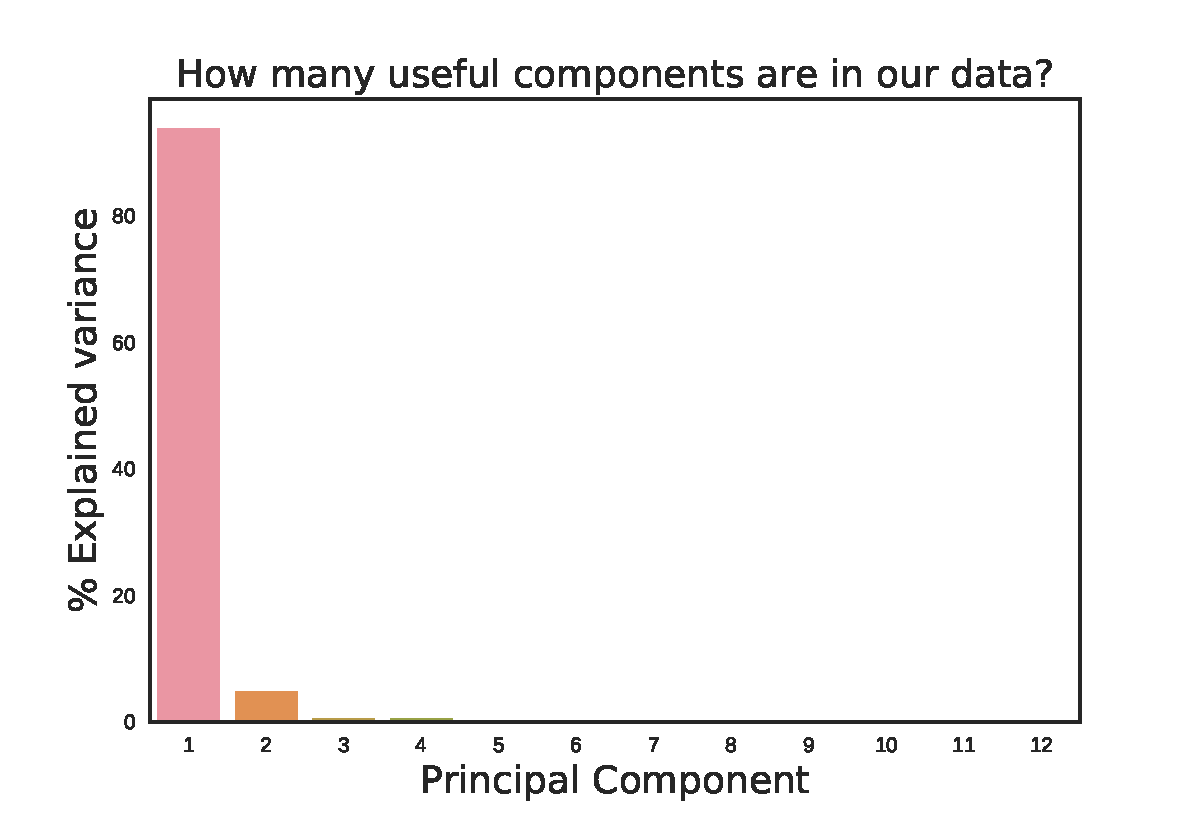
\includegraphics[width=185mm]{../Plots/ch_intro/pca_intro.pdf}
  \centering
  \caption{Explained variance decline for principal component analysis performed on a set of 12 all-sky infrared maps. The first three components account for over 99\% of the total variance. The PCA fit is performed on the whole sky, after whitening the data, using the ``scikitlearn }
\end{figure*}
